% Aspectratio 16:9 should be used
% The theme is not suited for 4:3 aspectratio
\documentclass[aspectratio=169]{beamer}
% Load the UGent theme
\usetheme[language=en,faculty=bw,usecolors]{ugent}
\usepackage[ugent]{timscolours}
\usepackage{svg}
\usepackage{graphicx} % Required for inserting images
\usepackage{pgfplots}
\pgfplotsset{compat=1.18}
% Packages
\usepackage[T1]{fontenc}
\usepackage[utf8]{inputenc}
\usepackage[english]{babel}
\usepackage{url,float,geometry,tikz,graphicx}
\usepackage{mathtools}
\usepackage{amsmath,amsthm,amsfonts,amssymb}
\usepackage{fancyhdr}
\usepackage{graphicx}
\usepackage{caption}
\usepackage{subcaption}
\usepackage{xcolor}
\usepackage{booktabs}
\usepackage{hyperref}
\usepackage{tikz-network}
\usepackage{mfirstuc}
\usepackage{environ}

% Control tikz compilation
\newif\ifhidetikz%
\hidetikzfalse%
%% Uncomment for faster compilation
% \hidetikztrue%

\ifhidetikz\RenewEnviron{tikzpicture}[1][]{%
	Tikz placeholder
}\fi

% Operators
\renewcommand{\vec}[1]{\mathbf{#1}}

\DeclareMathOperator*{\argmax}{arg\,max}
\DeclareMathOperator*{\argmin}{arg\,min}
\newcommand{\diag}[1]{\operatorname{diag} (#1)}

\newcommand{\mean}[1]{\left\langle\ #1 \right\rangle}

% Derivatives
\renewcommand{\d}{\mathrm{d}}
\newcommand{\dd}[2]{\frac{\d #1}{\d #2}}
\newcommand{\ddt}[1]{\dd{#1}{t}}

% Sets
\newcommand{\R}{\mathbb{R}}
\newcommand{\Rv}[1]{\R^#1}
\newcommand{\Rm}[2]{\R^{#1\times#2}}
\newcommand{\Rn}{\Rv{n}}
\newcommand{\Rnn}{\Rm{n}{n}}
\newcommand{\Rmn}{\Rm{m}{n}}

\newcommand{\Vs}{\mathcal{V}}
\newcommand{\Es}{\mathcal{E}}

% Neighbours
\newcommand{\nb}{k_i}
\newcommand{\nbs}[1]{{\nb^{#1}}}
\newcommand{\nbsI}{\nbs{I}}
\newcommand{\nbsA}{\nbs{A}}
\newcommand{\Nbh}{\mathcal{N}}
\newcommand{\Nbhi}{\Nbh_i}
\newcommand{\Nbhj}{\Nbh_j}

% LuMV parameters
\newcommand{\Dt}{\tau} % Time step
\newcommand{\Rinf}{\lambda} % infection rate
\newcommand{\Rrec}{\mu} % recovery rate
\newcommand{\Pinf}{\beta} % probability of infection
\newcommand{\Prec}{\gamma} % probability of recovery
\newcommand{\thres}{\Theta} %threshold
\newcommand{\comb}{\alpha} % combination parameter
\newcommand{\npi}{\eta} % Non-pharmaceutical interventions effect
\newcommand{\N}{N} % population size
\newcommand{\Pc}{\Pinf_c}
\newcommand{\Pstar}{\Pinf^*} % Equivalent transmission
\newcommand{\grf}{\delta}  % global reduction factor

% LuMV functions
\newcommand{\Pit}[2]{P_i^{#1\rightarrow~#2}}
\newcommand{\Ca}{C_\alpha(i)}
\newcommand{\Cua}{C^U_\alpha(v_i)}
\newcommand{\Caa}{C^A_\alpha(v_i)}
\newcommand{\Ea}{E_{\alpha_1\alpha_2} (v_i)}
\newcommand{\La}{L_{\alpha} (v_i)}

\renewcommand{\t}{(t)}
\newcommand{\tp}{(t+\tau)}
\newcommand{\tm}{(t-\tau)}

\newcommand{\pis}[1]{p_i^{#1}}
\newcommand{\pist}[1]{p_i^{#1}\t{}}

% Abbreviation or not?
\newcommand{\useabbreviations}{%
	\newcommand{\Fig}{Fig.}
	\newcommand{\Figs}{Figs.}
	\newcommand{\Tab}{Tab.}
	\newcommand{\Tabs}{Tabs.}
	\newcommand{\Eq}{Eq.}
	\newcommand{\Eqs}{Eqs.}
	\newcommand{\Sec}{Sec.}
	\newcommand{\Secs}{Secs.}

	\newcommand{\SW}{SW}
	\newcommand{\SF}{SF}
	\newcommand{\SWSF}{SW-SF}
	\newcommand{\SFSW}{SF-SW}
}

\newcommand{\usefull}{%
	\newcommand{\Fig}{Figure}
	\newcommand{\Figs}{Figures}
	\newcommand{\Tab}{Table}
	\newcommand{\Tabs}{Tables}
	\newcommand{\Eq}{Equation}
	\newcommand{\Eqs}{Equations}
	\newcommand{\Sec}{Section}
	\newcommand{\Secs}{Sections}

	\newcommand{\SW}{small-world}
	\newcommand{\SF}{scale-free}
	\newcommand{\SWSF}{small-world-scale-free}
	\newcommand{\SFSW}{scale-free-small-world}
}

% Julia Tikz preamble
\usetikzlibrary{arrows.meta}
\usetikzlibrary{backgrounds}
\usepgfplotslibrary{patchplots}
\usepgfplotslibrary{fillbetween}
\pgfplotsset{%
	    layers/standard/.define layer set={%
		        background,axis background,axis grid,axis ticks,axis lines,axis tick labels,pre main,main,axis descriptions,axis foreground%
		    }{%
		        grid style={/pgfplots/on layer=axis grid},%
		        tick style={/pgfplots/on layer=axis ticks},%
		        axis line style={/pgfplots/on layer=axis lines},%
		        label style={/pgfplots/on layer=axis descriptions},%
		        legend style={/pgfplots/on layer=axis descriptions},%
		        title style={/pgfplots/on layer=axis descriptions},%
		        colorbar style={/pgfplots/on layer=axis descriptions},%
		        ticklabel style={/pgfplots/on layer=axis tick labels},%
		        axis background@ style={/pgfplots/on layer=axis background},%
		        3d box foreground style={/pgfplots/on layer=axis foreground},%
		    },
	}

\usepgfplotslibrary{dateplot}
\usepgfplotslibrary{statistics}
\usetikzlibrary{pgfplots.colorbrewer}
\usepgfplotslibrary{fillbetween}

\usepackage{dirtree}
\renewcommand*\DTstylecomment{\small\textit}
\renewcommand*\DTstyle{\small}


\newcommand{\ymin}{0}
\newcommand{\ymax}{330}

\colorlet{color1}{ugentblue}
\colorlet{color2}{ugent-bw}
\colorlet{negcolor}{ugent-ge}

\colorlet{color1bw}{black!60}
\colorlet{color2bw}{black!30}
\colorlet{negcolorbw}{black!40}


\pgfplotsset{%
  colormap={divgrad}{%
    rgb(0.00000000)=(0.81882353,0.33176471,0.39882353)
    rgb(0.50000000)=(1.00000000,1.00000000,1.00000000)
    rgb(1.00000000)=(0.10588235,0.35294118,0.70588235)
  },
  colormap={linear}{%
    rgb(0.00000000)=(1.00000000,1.00000000,1.00000000)
    rgb(1.00000000)=(0.10588235,0.35294118,0.70588235)
  },
}

\usetikzlibrary{external}
%\tikzexternalize[prefix=figures/]

\pgfplotsset{%
  timeseries/.style={%
    width=.95\textwidth,
    height=100pt,
    %
    date coordinates in = x,
    xmin=2019-12-01,
    xmax=2022-06-30,
    xtick={2020-01-01,2020-07-01,2021-01-01,2021-07-01,2022-01-01},
    xticklabels={},
    %
    ymin=\ymin,
    ylabel style={align=center},
    yticklabel style={%
      text width=20pt,
      align=right
    },
    %
    axis lines*=left,
    x axis line style={white},
    x tick style={lightgray},
    xmajorgrids=true,
    grid style={lightgray},
  },
  %
  commentseries/.style={%
    timeseries,
    ymax=\ymax,
    ytick={0,100,200,300},
  },
  %
  tsdates/.style={%
    xticklabels={2020-01-01,2020-07-01,2021-01-01,2021-07-01,2022-01-01,2022-07-01},
    xticklabel=\year-\month,
  },
  %
  tsline/.style={%
    mark=none,
    line width=1pt,
  },
}

\newcommand{\negativeday}[2][negcolor]{%
  \addplot[line width=1pt, color=#1] coordinates {(#2, \ymin) (#2, \ymax)};
}

\newcommand{\addperiod}[4][color2]{%
  \fill[#1, opacity=0.3] (axis cs: #3,\ymin) rectangle (axis cs: #4,\pgfkeysvalueof{/pgfplots/ymax});
  \node[anchor=north west, rotate=-90] at (axis cs: #3, \pgfkeysvalueof{/pgfplots/ymax}) {\scriptsize #2};
}

\newcommand{\addtrend}[2][color1]{%
  \addplot[tsline, color=#1, dashed] table[x=date, y=vals, col sep=comma]{input/timeseries/belgium_#2_trend.csv};
}

\newcommand{\addevent}[6][color2]{%
  \addplot[tsline, #1] coordinates {(#3, #4) (#5, #2)};
    \node[anchor=south,align=center,text=color2,font=\scriptsize] at (axis cs: #5, #2) {#6};
}

\newcommand{\timeseries}[5][]{%
    \begin{axis}[
        commentseries,
        ylabel={\color{#4}#3},
        #1,
      ]
      #5;
      %\addtrend{#2}
      \addplot[tsline, color=#4] table[x=date, y=nb_posts, col sep=comma]{figures/timeseries/belgium_#2.csv};
    \end{axis}
}

\newcommand{\focusedlockdown}{%
  \timeseries[tsdates]{lockdown}{Lockdowns}{color1}{%
    \addperiod[color2]{}{2020-03-13}{2020-06-08}
    \addperiod[color2]{}{2020-07-29}{2020-08-26}
    \addperiod[color2]{}{2020-10-19}{2021-06-09}
    \addperiod[color2]{}{2021-11-27}{2022-02-18}
    \negativeday[negcolor]{2020-03-14}
    \negativeday[negcolor]{2021-01-21}
    \negativeday[negcolor]{2022-05-25}
  }
}

\newcommand{\unfocusedlockdown}{%
  \timeseries{lockdown}{Lockdowns}{color1bw}{%
    \negativeday[negcolorbw]{2020-03-14}
    \negativeday[negcolorbw]{2021-01-21}
    \negativeday[negcolorbw]{2022-05-25}
  }
}

\newcommand{\focusedmask}{%
  \timeseries[yshift=-80pt, tsdates]{mask}{Masks}{color1}{%
    \negativeday[negcolor]{2020-07-09}
    \negativeday[negcolor]{2020-10-27}
    \negativeday[negcolor]{2020-11-21}
    \negativeday[negcolor]{2021-04-18}
    \negativeday[negcolor]{2022-01-15}
    \addevent{200}{2020-07-09}{130}{2020-05-27}{General \\ mandate}
    \addevent{150}{2021-09-17}{60}{2021-06-15}{End in \\ Flanders}
    \addevent{200}{2021-11-17}{110}{2021-10-01}{Broad \\ reintroduction}
  }
}

\newcommand{\unfocusedmask}{%
  \timeseries[yshift=-80pt]{mask}{Masks}{color1bw}{%
    \negativeday[negcolorbw]{2020-07-09}
    \negativeday[negcolorbw]{2020-10-27}
    \negativeday[negcolorbw]{2020-11-21}
    \negativeday[negcolorbw]{2021-04-18}
    \negativeday[negcolorbw]{2022-01-15}
  }
}

\newcommand{\focusedvaccin}{%
  \timeseries[yshift=-160pt, tsdates]{vaccin}{Vaccination}{color1}{%
      \addevent{200}{2020-12-28}{130}{2020-11-16}{Start campaign}
      \addevent{200}{2021-11-01}{140}{2021-09-16}{Healthcare \\ obligation}
      \negativeday[negcolor]{2020-09-03}
    }
}

\newcommand{\unfocusedvaccin}{%
  \timeseries[yshift=-160pt]{vaccin}{Vaccination}{color1bw}{%
      \negativeday[negcolorbw]{2020-09-03}
    }
}


%% HEATMAPS!

\pgfplotsset{%
  heatmap/.style={%
    width=.75\textwidth,
    height=.75\textwidth,
    point meta=explicit,
    %
    xmin=-1.025,
    xmax=1.025,
    xlabel={Sentiment of comment},
    xtick={-1.0, 0.0, 1.0},
    %
    ymin=-1.025,
    ymax=1.025,
    ylabel={Sentiment of parent},
    ylabel style={%
      yshift=-7pt
    },
    ytick={-1.0, 0.0, 1.0},
    %
    colorbar,
  },
  %
  sentheatmap/.style={%
    heatmap,
    colormap name={linear},
    point meta min=0.0,
    point meta max=2.5,
    colorbar style={%
      samples=3,
      scaled y ticks=false,
      ytick={0, 2.2},
      yticklabels={None, Many},
    },
  },
  %
  diffheatmap/.style={%
    heatmap,
    colormap name={divgrad},
    point meta min=-1.15,
    point meta max=1.15,
    colorbar style={%
      samples=3,
      scaled y ticks=false,
      ytick={{-1, 0, 1}},
      yticklabels={{Less, Expected, More}},
    },
  },
  %
  plotheatmap/.style={%
    matrix plot*,
    mesh/cols=41,
    point meta=explicit,
  }
}

\newcommand{\sentheatmap}[2][]{%
  \begin{axis}[sentheatmap,#1]
    \addplot [plotheatmap] table [x=x, y=y, meta=z, col sep=comma] {figures/sentiment/belgium_#2_bert_sent.csv};
  \end{axis}
}

\newcommand{\diffheatmap}[2][]{%
  \begin{axis}[diffheatmap,#1]
    \addplot [plotheatmap] table [x=x, y=y, meta=z, col sep=comma] {figures/sentiment/belgium_#2_bert_diff.csv};
  \end{axis}
}

%% Ze network


\newcommand{\vertextree}{%
  \SetVertexStyle[LineWidth=0pt]
  \Vertex[x=0,y=0,color=negcolor,]{T}

  \Vertex[x=-1.5,y=-1.25,color=negcolor,]{S1}
  \Vertex[x=0,y=-1.25,color=negcolor,]{S2}
  \Vertex[x=1.5,y=-1.25,color=color2,]{S3}

  \Vertex[x=-2.25,y=-2.5,color=negcolor,]{T1}
  \Vertex[x=-.75,y=-2.5,color=negcolor,]{T2}
  \Vertex[x=0.75,y=-2.5,color=color2,]{T3}
  \Vertex[x=2.25,y=-2.5,color=negcolor,]{T4}

  \Vertex[x=-.75,y=-3.75,color=negcolor,]{F5}
}

\newcommand{\structurededges}{%
  \Edge[Direct](S1)(T)
  \Edge[Direct](S2)(T)
  \Edge[Direct](S3)(T)

  \Edge[Direct](T1)(S2)
  \Edge[Direct](T2)(S2)
  \Edge[Direct](T3)(S3)
  \Edge[Direct](T4)(S3)

  \Edge[Direct](F5)(T2)
}

\newcommand{\randomedges}{%
  \Edge[Direct](S1)(S2)
  \Edge[Direct](S2)(T1)
  \Edge[Direct](S3)(S2)

  \Edge[Direct](T1)(T2)
  \Edge[Direct](T2)(S1)
  \Edge[Direct](T3)(T)
  \Edge[Direct](T4)(T)

  \Edge[Direct](F5)(T2)
}

%% Homophily curve
\pgfplotsset{%
  homo/.style={%
    width = .9\textwidth,
    height = .75\textwidth,
    %
    xmin=1,
    xmax=5,
    xlabel={context size \( n \)},
    %
    ymin=0,
    ymax=0.28,
    scaled y ticks=false,
    ytick={0,.1,.2},
    yticklabels={},
    %
    legend style={%
      at={(0.95,0.95)},
      anchor=north east,
    },
    reverse legend,
  },
  %
  homoylabels/.style={%
    ylabel={homophily},
    yticklabels={0,0.1,0.2},
  },
  %
  homoline/.style={%
    mark=none,
    line width=2pt,
  },
  %
}

\newcommand{\addhomolegend}{%
  \legend{\( U^n \), \( A^n \)};
}

\newcommand{\sentimenthomophily}[4][]{%
  \begin{axis}[homo, #1]
    \addplot[
      homoline, color1, mark=*,
      restrict x to domain=1:#3,
    ] table[x=x, y=gen, col sep=comma]{figures/sentiment/belgium_#2_bert_context.csv};
    \addplot[
      homoline, color2, mark=*,
      restrict x to domain=1:#4,
    ] table[x=x, y=prev_parent, col sep=comma]{figures/sentiment/belgium_#2_bert_context.csv};
  \end{axis}
}

%% User context
\newcommand{\commenttree}[1]{%
  \node at (0,0) {%
    \begin{minipage}[t]{\textwidth}
      \dirtree{%
        .1 \color{color1\ifnum#1<5 bw\fi} Ancestor submission or comment.
          .2 \color{color1\ifnum#1<4 bw\fi} Ancestor comment.
            .3 \color{color1\ifnum#1<3 bw\fi} Ancestor comment.
              .4 \color{color1\ifnum#1<2 bw\fi} Ancestor comment.
                .5 \color{color1\ifnum#1<1 bw\fi} Parent comment.
                  .6 Reference comment.
      }
    \end{minipage}
  };
}

\newcommand{\commenttimeline}[1]{%
  \draw[->] (-4.25,5.5) -- (-4.25,-0.5) node[right] {$t$};

  \node at (0,0){%
      \begin{minipage}[t]{\textwidth}
        \dirtree{%
          .1 \color{color2} Parent comment.
            .2 Reference comment.
        }
      \end{minipage}
    };

  \foreach \i in {1,2,3,4} {
    \def\yfactors{{1.25, 2.3, 3.9, 5.1}}
      \pgfmathsetmacro{\y}{\yfactors[\i-1]}
      \pgfmathtruncatemacro{\j}{\i + 1}
      \node at (0,\y){%
        \begin{minipage}[t]{\textwidth}
        \dirtree{%
          .1 \color{color2\ifnum#1<\j bw\fi} Parent comment.
          .2 \color{\ifnum#1<\j black!60\else black\fi} Comment by same user.
        }
        \end{minipage}
      };
  }
}

%% Sentiment distributions
\pgfplotsset{%
  model/.style={%
    width=1.25\textwidth,
    %
    axis lines*=left,
    %
    xmin=-1.05,
    xmax=1.05,
    xlabel={\( s \)},
    %
    ymin=0,
    ymax=1.4,
    ytick=\empty,
    yticklabels={},
    y axis line style={opacity=0},
    %
    legend style={%
      at={(0.95,1.)},
      anchor=north east,
      draw=none,
      font=\scriptsize,
    },
  },
  %
  modelhist/.style={%
    ybar,
    bar width=0.05,
    fill,
    fill opacity = 0.75,
    mark=none,
    draw=none,
  },
  %
  alphahist/.style={%
    ybar,
    bar width=0.137931,
    mark=none,
    fill,
    fill opacity=0.75,
    draw=none,
  },
}

\newcommand{\addmodellegend}{%
  \addlegendimage{area legend, color1, opacity=0.75, fill=color1, fill opacity=0.75};
  \addlegendentry{Predicted};
  \addlegendimage{area legend, color2, opacity=0.75, fill=color2, fill opacity=0.75};
  \addlegendentry{Observed};
}

\newcommand{\modelsentiment}[3][]{%
  \begin{axis}[model, #1]
    #3
    \addplot[modelhist, color1, fill] table[x=x, y=y_pred, col sep=comma]{figures/siebc/belgium_#2_histogram.csv};
    \addplot[modelhist, color2] table[x=x, y=y_obs, col sep=comma]{figures/siebc/belgium_#2_histogram.csv};
  \end{axis}
}

\newcommand{\singletopic}[1]{%
  \addplot+[
        boxplot,
        black,
        line width=2pt,
        mark=none,
      ]
      table[y=#1, col sep=comma] {figures/siebc/belgium_homophily.csv};
}

\newcommand{\refline}[3]{%
  \draw[black, dashed, line width=2pt] (axis cs:#1,#3) -- (axis cs:#2,#3);
}

\newcommand{\homophilyboxplot}[1][]{%
  \begin{axis}[
    #1,
    width=0.45\textwidth,
    %
    xtick={1,2,3},
    xticklabels={Lockdown, Mask, Vaccin},
    %
    ymin=0.,
    ylabel=\( h(\Delta H^s) \),
    %
    axis lines*=left,
    x axis line style={draw=none},
    x tick style={draw=none},
    %
    boxplot/draw direction=y,
  ]
    \singletopic{lockdown}
    \singletopic{mask}
    \singletopic{vaccin}
    \refline{.6}{1.4}{0.20490}
    \refline{1.6}{2.4}{0.22200}
    \refline{2.6}{3.4}{0.14807}
  \end{axis}
}

\newcommand{\alphaslegend}{%
  \addlegendimage{area legend, color1, opacity=0.75, fill=color1, fill opacity=0.75};
  \addlegendentry{\( \alpha_u \)};
  \addlegendimage{area legend, color2, opacity=0.75, fill=color2, fill opacity=0.75};
  \addlegendentry{\( \alpha_e \)};
  \addlegendimage{densely dashed, line width=1.5pt}
  \addlegendentry{mean}
}

\newcommand{\modelalphas}[5][]{%
  \begin{axis}[
    width=1.25\textwidth,
    % %
    axis lines*=left,
    % %
    xmin=-0.05,
    xmax=4.05,
    xlabel={\( \alpha \)},
    % %
    ymin=0.0,
    ymax=0.525,
    ytick=\empty,
    yticklabels={},
    y axis line style={opacity=0},
    % %
    legend style={%
      at={(0.95,1.)},
      anchor=north east,
      draw=none,
      font=\scriptsize,
    },
  ]
    #5
    \addplot[alphahist, color1] table[x=x, y=a1, col sep=comma]{figures/siebc/#2_alpha_hist.csv};
    \addplot[alphahist, color2] table[x=x, y=a2, col sep=comma]{figures/siebc/#2_alpha_hist.csv};
    \addplot[draw=color1, densely dashed, line width=1.5pt] coordinates {(#3,0) (#3,0.475)};
    \addplot[draw=color2, densely dashed, line width=1.5pt] coordinates {(#4,0) (#4,0.475)};
  \end{axis}
}



%\usepgfplotslibrary{dateplot}
\usepgfplotslibrary{statistics}
\usetikzlibrary{pgfplots.colorbrewer}
\usepgfplotslibrary{fillbetween}

\usepackage{dirtree}
\renewcommand*\DTstylecomment{\small\textit}
\renewcommand*\DTstyle{\small}


\newcommand{\ymin}{0}
\newcommand{\ymax}{330}

\colorlet{color1}{ugentblue}
\colorlet{color2}{ugent-bw}
\colorlet{negcolor}{ugent-ge}

\colorlet{color1bw}{black!60}
\colorlet{color2bw}{black!30}
\colorlet{negcolorbw}{black!40}


\pgfplotsset{%
  colormap={divgrad}{%
    rgb(0.00000000)=(0.81882353,0.33176471,0.39882353)
    rgb(0.50000000)=(1.00000000,1.00000000,1.00000000)
    rgb(1.00000000)=(0.10588235,0.35294118,0.70588235)
  },
  colormap={linear}{%
    rgb(0.00000000)=(1.00000000,1.00000000,1.00000000)
    rgb(1.00000000)=(0.10588235,0.35294118,0.70588235)
  },
}

\usetikzlibrary{external}
%\tikzexternalize[prefix=figures/]

\pgfplotsset{%
  timeseries/.style={%
    width=.95\textwidth,
    height=100pt,
    %
    date coordinates in = x,
    xmin=2019-12-01,
    xmax=2022-06-30,
    xtick={2020-01-01,2020-07-01,2021-01-01,2021-07-01,2022-01-01},
    xticklabels={},
    %
    ymin=\ymin,
    ylabel style={align=center},
    yticklabel style={%
      text width=20pt,
      align=right
    },
    %
    axis lines*=left,
    x axis line style={white},
    x tick style={lightgray},
    xmajorgrids=true,
    grid style={lightgray},
  },
  %
  commentseries/.style={%
    timeseries,
    ymax=\ymax,
    ytick={0,100,200,300},
  },
  %
  tsdates/.style={%
    xticklabels={2020-01-01,2020-07-01,2021-01-01,2021-07-01,2022-01-01,2022-07-01},
    xticklabel=\year-\month,
  },
  %
  tsline/.style={%
    mark=none,
    line width=1pt,
  },
}

\newcommand{\negativeday}[2][negcolor]{%
  \addplot[line width=1pt, color=#1] coordinates {(#2, \ymin) (#2, \ymax)};
}

\newcommand{\addperiod}[4][color2]{%
  \fill[#1, opacity=0.3] (axis cs: #3,\ymin) rectangle (axis cs: #4,\pgfkeysvalueof{/pgfplots/ymax});
  \node[anchor=north west, rotate=-90] at (axis cs: #3, \pgfkeysvalueof{/pgfplots/ymax}) {\scriptsize #2};
}

\newcommand{\addtrend}[2][color1]{%
  \addplot[tsline, color=#1, dashed] table[x=date, y=vals, col sep=comma]{input/timeseries/belgium_#2_trend.csv};
}

\newcommand{\addevent}[6][color2]{%
  \addplot[tsline, #1] coordinates {(#3, #4) (#5, #2)};
    \node[anchor=south,align=center,text=color2,font=\scriptsize] at (axis cs: #5, #2) {#6};
}

\newcommand{\timeseries}[5][]{%
    \begin{axis}[
        commentseries,
        ylabel={\color{#4}#3},
        #1,
      ]
      #5;
      %\addtrend{#2}
      \addplot[tsline, color=#4] table[x=date, y=nb_posts, col sep=comma]{figures/timeseries/belgium_#2.csv};
    \end{axis}
}

\newcommand{\focusedlockdown}{%
  \timeseries[tsdates]{lockdown}{Lockdowns}{color1}{%
    \addperiod[color2]{}{2020-03-13}{2020-06-08}
    \addperiod[color2]{}{2020-07-29}{2020-08-26}
    \addperiod[color2]{}{2020-10-19}{2021-06-09}
    \addperiod[color2]{}{2021-11-27}{2022-02-18}
    \negativeday[negcolor]{2020-03-14}
    \negativeday[negcolor]{2021-01-21}
    \negativeday[negcolor]{2022-05-25}
  }
}

\newcommand{\unfocusedlockdown}{%
  \timeseries{lockdown}{Lockdowns}{color1bw}{%
    \negativeday[negcolorbw]{2020-03-14}
    \negativeday[negcolorbw]{2021-01-21}
    \negativeday[negcolorbw]{2022-05-25}
  }
}

\newcommand{\focusedmask}{%
  \timeseries[yshift=-80pt, tsdates]{mask}{Masks}{color1}{%
    \negativeday[negcolor]{2020-07-09}
    \negativeday[negcolor]{2020-10-27}
    \negativeday[negcolor]{2020-11-21}
    \negativeday[negcolor]{2021-04-18}
    \negativeday[negcolor]{2022-01-15}
    \addevent{200}{2020-07-09}{130}{2020-05-27}{General \\ mandate}
    \addevent{150}{2021-09-17}{60}{2021-06-15}{End in \\ Flanders}
    \addevent{200}{2021-11-17}{110}{2021-10-01}{Broad \\ reintroduction}
  }
}

\newcommand{\unfocusedmask}{%
  \timeseries[yshift=-80pt]{mask}{Masks}{color1bw}{%
    \negativeday[negcolorbw]{2020-07-09}
    \negativeday[negcolorbw]{2020-10-27}
    \negativeday[negcolorbw]{2020-11-21}
    \negativeday[negcolorbw]{2021-04-18}
    \negativeday[negcolorbw]{2022-01-15}
  }
}

\newcommand{\focusedvaccin}{%
  \timeseries[yshift=-160pt, tsdates]{vaccin}{Vaccination}{color1}{%
      \addevent{200}{2020-12-28}{130}{2020-11-16}{Start campaign}
      \addevent{200}{2021-11-01}{140}{2021-09-16}{Healthcare \\ obligation}
      \negativeday[negcolor]{2020-09-03}
    }
}

\newcommand{\unfocusedvaccin}{%
  \timeseries[yshift=-160pt]{vaccin}{Vaccination}{color1bw}{%
      \negativeday[negcolorbw]{2020-09-03}
    }
}


%% HEATMAPS!

\pgfplotsset{%
  heatmap/.style={%
    width=.75\textwidth,
    height=.75\textwidth,
    point meta=explicit,
    %
    xmin=-1.025,
    xmax=1.025,
    xlabel={Sentiment of comment},
    xtick={-1.0, 0.0, 1.0},
    %
    ymin=-1.025,
    ymax=1.025,
    ylabel={Sentiment of parent},
    ylabel style={%
      yshift=-7pt
    },
    ytick={-1.0, 0.0, 1.0},
    %
    colorbar,
  },
  %
  sentheatmap/.style={%
    heatmap,
    colormap name={linear},
    point meta min=0.0,
    point meta max=2.5,
    colorbar style={%
      samples=3,
      scaled y ticks=false,
      ytick={0, 2.2},
      yticklabels={None, Many},
    },
  },
  %
  diffheatmap/.style={%
    heatmap,
    colormap name={divgrad},
    point meta min=-1.15,
    point meta max=1.15,
    colorbar style={%
      samples=3,
      scaled y ticks=false,
      ytick={{-1, 0, 1}},
      yticklabels={{Less, Expected, More}},
    },
  },
  %
  plotheatmap/.style={%
    matrix plot*,
    mesh/cols=41,
    point meta=explicit,
  }
}

\newcommand{\sentheatmap}[2][]{%
  \begin{axis}[sentheatmap,#1]
    \addplot [plotheatmap] table [x=x, y=y, meta=z, col sep=comma] {figures/sentiment/belgium_#2_bert_sent.csv};
  \end{axis}
}

\newcommand{\diffheatmap}[2][]{%
  \begin{axis}[diffheatmap,#1]
    \addplot [plotheatmap] table [x=x, y=y, meta=z, col sep=comma] {figures/sentiment/belgium_#2_bert_diff.csv};
  \end{axis}
}

%% Ze network


\newcommand{\vertextree}{%
  \SetVertexStyle[LineWidth=0pt]
  \Vertex[x=0,y=0,color=negcolor,]{T}

  \Vertex[x=-1.5,y=-1.25,color=negcolor,]{S1}
  \Vertex[x=0,y=-1.25,color=negcolor,]{S2}
  \Vertex[x=1.5,y=-1.25,color=color2,]{S3}

  \Vertex[x=-2.25,y=-2.5,color=negcolor,]{T1}
  \Vertex[x=-.75,y=-2.5,color=negcolor,]{T2}
  \Vertex[x=0.75,y=-2.5,color=color2,]{T3}
  \Vertex[x=2.25,y=-2.5,color=negcolor,]{T4}

  \Vertex[x=-.75,y=-3.75,color=negcolor,]{F5}
}

\newcommand{\structurededges}{%
  \Edge[Direct](S1)(T)
  \Edge[Direct](S2)(T)
  \Edge[Direct](S3)(T)

  \Edge[Direct](T1)(S2)
  \Edge[Direct](T2)(S2)
  \Edge[Direct](T3)(S3)
  \Edge[Direct](T4)(S3)

  \Edge[Direct](F5)(T2)
}

\newcommand{\randomedges}{%
  \Edge[Direct](S1)(S2)
  \Edge[Direct](S2)(T1)
  \Edge[Direct](S3)(S2)

  \Edge[Direct](T1)(T2)
  \Edge[Direct](T2)(S1)
  \Edge[Direct](T3)(T)
  \Edge[Direct](T4)(T)

  \Edge[Direct](F5)(T2)
}

%% Homophily curve
\pgfplotsset{%
  homo/.style={%
    width = .9\textwidth,
    height = .75\textwidth,
    %
    xmin=1,
    xmax=5,
    xlabel={context size \( n \)},
    %
    ymin=0,
    ymax=0.28,
    scaled y ticks=false,
    ytick={0,.1,.2},
    yticklabels={},
    %
    legend style={%
      at={(0.95,0.95)},
      anchor=north east,
    },
    reverse legend,
  },
  %
  homoylabels/.style={%
    ylabel={homophily},
    yticklabels={0,0.1,0.2},
  },
  %
  homoline/.style={%
    mark=none,
    line width=2pt,
  },
  %
}

\newcommand{\addhomolegend}{%
  \legend{\( U^n \), \( A^n \)};
}

\newcommand{\sentimenthomophily}[4][]{%
  \begin{axis}[homo, #1]
    \addplot[
      homoline, color1, mark=*,
      restrict x to domain=1:#3,
    ] table[x=x, y=gen, col sep=comma]{figures/sentiment/belgium_#2_bert_context.csv};
    \addplot[
      homoline, color2, mark=*,
      restrict x to domain=1:#4,
    ] table[x=x, y=prev_parent, col sep=comma]{figures/sentiment/belgium_#2_bert_context.csv};
  \end{axis}
}

%% User context
\newcommand{\commenttree}[1]{%
  \node at (0,0) {%
    \begin{minipage}[t]{\textwidth}
      \dirtree{%
        .1 \color{color1\ifnum#1<5 bw\fi} Ancestor submission or comment.
          .2 \color{color1\ifnum#1<4 bw\fi} Ancestor comment.
            .3 \color{color1\ifnum#1<3 bw\fi} Ancestor comment.
              .4 \color{color1\ifnum#1<2 bw\fi} Ancestor comment.
                .5 \color{color1\ifnum#1<1 bw\fi} Parent comment.
                  .6 Reference comment.
      }
    \end{minipage}
  };
}

\newcommand{\commenttimeline}[1]{%
  \draw[->] (-4.25,5.5) -- (-4.25,-0.5) node[right] {$t$};

  \node at (0,0){%
      \begin{minipage}[t]{\textwidth}
        \dirtree{%
          .1 \color{color2} Parent comment.
            .2 Reference comment.
        }
      \end{minipage}
    };

  \foreach \i in {1,2,3,4} {
    \def\yfactors{{1.25, 2.3, 3.9, 5.1}}
      \pgfmathsetmacro{\y}{\yfactors[\i-1]}
      \pgfmathtruncatemacro{\j}{\i + 1}
      \node at (0,\y){%
        \begin{minipage}[t]{\textwidth}
        \dirtree{%
          .1 \color{color2\ifnum#1<\j bw\fi} Parent comment.
          .2 \color{\ifnum#1<\j black!60\else black\fi} Comment by same user.
        }
        \end{minipage}
      };
  }
}

%% Sentiment distributions
\pgfplotsset{%
  model/.style={%
    width=1.25\textwidth,
    %
    axis lines*=left,
    %
    xmin=-1.05,
    xmax=1.05,
    xlabel={\( s \)},
    %
    ymin=0,
    ymax=1.4,
    ytick=\empty,
    yticklabels={},
    y axis line style={opacity=0},
    %
    legend style={%
      at={(0.95,1.)},
      anchor=north east,
      draw=none,
      font=\scriptsize,
    },
  },
  %
  modelhist/.style={%
    ybar,
    bar width=0.05,
    fill,
    fill opacity = 0.75,
    mark=none,
    draw=none,
  },
  %
  alphahist/.style={%
    ybar,
    bar width=0.137931,
    mark=none,
    fill,
    fill opacity=0.75,
    draw=none,
  },
}

\newcommand{\addmodellegend}{%
  \addlegendimage{area legend, color1, opacity=0.75, fill=color1, fill opacity=0.75};
  \addlegendentry{Predicted};
  \addlegendimage{area legend, color2, opacity=0.75, fill=color2, fill opacity=0.75};
  \addlegendentry{Observed};
}

\newcommand{\modelsentiment}[3][]{%
  \begin{axis}[model, #1]
    #3
    \addplot[modelhist, color1, fill] table[x=x, y=y_pred, col sep=comma]{figures/siebc/belgium_#2_histogram.csv};
    \addplot[modelhist, color2] table[x=x, y=y_obs, col sep=comma]{figures/siebc/belgium_#2_histogram.csv};
  \end{axis}
}

\newcommand{\singletopic}[1]{%
  \addplot+[
        boxplot,
        black,
        line width=2pt,
        mark=none,
      ]
      table[y=#1, col sep=comma] {figures/siebc/belgium_homophily.csv};
}

\newcommand{\refline}[3]{%
  \draw[black, dashed, line width=2pt] (axis cs:#1,#3) -- (axis cs:#2,#3);
}

\newcommand{\homophilyboxplot}[1][]{%
  \begin{axis}[
    #1,
    width=0.45\textwidth,
    %
    xtick={1,2,3},
    xticklabels={Lockdown, Mask, Vaccin},
    %
    ymin=0.,
    ylabel=\( h(\Delta H^s) \),
    %
    axis lines*=left,
    x axis line style={draw=none},
    x tick style={draw=none},
    %
    boxplot/draw direction=y,
  ]
    \singletopic{lockdown}
    \singletopic{mask}
    \singletopic{vaccin}
    \refline{.6}{1.4}{0.20490}
    \refline{1.6}{2.4}{0.22200}
    \refline{2.6}{3.4}{0.14807}
  \end{axis}
}

\newcommand{\alphaslegend}{%
  \addlegendimage{area legend, color1, opacity=0.75, fill=color1, fill opacity=0.75};
  \addlegendentry{\( \alpha_u \)};
  \addlegendimage{area legend, color2, opacity=0.75, fill=color2, fill opacity=0.75};
  \addlegendentry{\( \alpha_e \)};
  \addlegendimage{densely dashed, line width=1.5pt}
  \addlegendentry{mean}
}

\newcommand{\modelalphas}[5][]{%
  \begin{axis}[
    width=1.25\textwidth,
    % %
    axis lines*=left,
    % %
    xmin=-0.05,
    xmax=4.05,
    xlabel={\( \alpha \)},
    % %
    ymin=0.0,
    ymax=0.525,
    ytick=\empty,
    yticklabels={},
    y axis line style={opacity=0},
    % %
    legend style={%
      at={(0.95,1.)},
      anchor=north east,
      draw=none,
      font=\scriptsize,
    },
  ]
    #5
    \addplot[alphahist, color1] table[x=x, y=a1, col sep=comma]{figures/siebc/#2_alpha_hist.csv};
    \addplot[alphahist, color2] table[x=x, y=a2, col sep=comma]{figures/siebc/#2_alpha_hist.csv};
    \addplot[draw=color1, densely dashed, line width=1.5pt] coordinates {(#3,0) (#3,0.475)};
    \addplot[draw=color2, densely dashed, line width=1.5pt] coordinates {(#4,0) (#4,0.475)};
  \end{axis}
}


%\usepgfplotslibrary{external}
%\tikzexternalize[prefix=figures/externalize/]
% Metadata of the presentation
\title{Coevolution of opinions and epidemics on networks.}
\date{26th February 2026}% \\ Tim Van Wesemael}
\author[TVW]{Tim Van Wesemael}

% Have this if you'd like section slides
\AtBeginSection[]{%
    \sectionframe%
}

\newcommand{\backupbegin}{%
	\newcounter{framenumberappendix}
	\setcounter{framenumberappendix}{\value{framenumber}}
}
\newcommand{\backupend}{%
	\addtocounter{framenumberappendix}{-\value{framenumber}}
	\addtocounter{framenumber}{\value{framenumberappendix}}
}

\newcommand{\graphwidth}{0.8\textwidth}
\newcommand{\graphlabelsize}{\small}
\newcommand{\ylabelshift}{-2pt}

\newcommand{\twocolumns}[3][.5]{%
  \begin{columns}
    \begin{column}{#1\textwidth}
      #2
    \end{column}
    \begin{column}{\dimexpr(\textwidth - #1\textwidth)\relax}
      #3
    \end{column}
  \end{columns}
}

\newcommand{\tabhead}[1]{\textbf{#1}}

\begin{document}

% Have this if you'd like the presentation to start
% with a large UGent logo
%\logoframe

% I guess you always want a titleframe
\titleframe


\begin{frame}{Social contagion}
	\begin{columns}
		\begin{column}{0.5\textwidth}
			\begin{itemize}
				\item Many social phenomena
					\begin{itemize}
						\item Ideas
						\item Memes
						\item Adoption of innovation
						\item ...
					\end{itemize}
				\item Diffusion or epidemic-like? (\emph{viral spread})
				\item<2-> In many ways not!
			\end{itemize}
		\end{column}
		\begin{column}{0.5\textwidth}
			\centering
			\includegraphics<1>[width=0.9\textwidth]{figures/pics/planking}
			\includegraphics<2>[width=0.9\textwidth]{figures/pics/vintage-planking}
		\end{column}
	\end{columns}
\end{frame}

\begin{frame}{Discrete opinion dynamics}
	\begin{itemize}
		\item Like magnets? Ising model!
		\item $H = -\sum_{i,j} J_{ij} \sigma_i \sigma_j - \mu\sum h_j \sigma_j$ with $\sigma_i \in \{-1, +1\}$
		\item Allows for microscopic interactions through $J_{ij}$
	\end{itemize}
	\begin{columns}
		\begin{column}{.33\textwidth}\centering\includegraphics[width=0.8\textwidth]{figures/pics/ising-1}\end{column}
		\begin{column}{.33\textwidth}\centering\includegraphics[width=0.8\textwidth]{figures/pics/ising-2}\end{column}
		\begin{column}{.33\textwidth}\centering\includegraphics[width=0.8\textwidth]{figures/pics/ising-3}\end{column}
	\end{columns}
\end{frame}

\begin{frame}{Discrete opinion dynamics}
	\begin{itemize}
		\item Or complex contagion?
		\item Interactions with the contagion are not independent
		\item Threshold model: adopt if number of contagious neighbours reach threshold
	\end{itemize}
	\centering
	\includegraphics[width=0.3\textwidth]{figures/pics/watts}
\end{frame}

\begin{frame}{Continuous opinion space}
	\begin{columns}
	\begin{column}{0.5\linewidth}
		Bounded confidence
		\begin{itemize}
			\item Diffusion-like
			\item Only adjust to opinion that is close enough to yours (< $\epsilon$)
			\item Fragmentation $\rightarrow$ polarization $\rightarrow$ consensus
		\end{itemize}
	\end{column}
	\begin{column}{0.5\linewidth}
		\centering
		\includegraphics[width=0.9\textwidth]{figures/pics/HK.png}
		(Hegselmann, 2002)
	\end{column}
	\end{columns}
\end{frame}

\begin{frame}{Data-driven approaches}
	\begin{itemize}
		\item Only a small fraction of models have been validated with empirical data
		\item Observationally, complex contagions have been identified, such as the adoptation of a politically motivated profile picture (State, 2015)
		\item Small-scale randomised experiments confirmed these results (Centola, 2015)
	\end{itemize}
	\vfill
	\centering
	\includegraphics[width=0.66\textwidth]{figures/pics/equality}
	\vfill
\end{frame}

\begin{frame}{Data-driven approaches}
	\begin{itemize}
		\item Only a small fraction of models have been validated with empirical data
		\item Observationally, complex contagions have been identified, such as the adoptation of a politically motivated profile picture (State, 2015)
		\item Small-scale randomised experiments confirmed these results (Centola, 2015)
	\end{itemize}
	\vfill
	\begin{columns}
		\begin{column}{0.33\textwidth}
			\centering
			Facebook \\
			\includegraphics[width=0.4\textwidth]{figures/valensise/fbo}
			\includegraphics[width=0.4\textwidth]{figures/valensise/fbs}
		\end{column}
		\begin{column}{0.33\textwidth}
			\centering
			Twitter \\
			\includegraphics[width=0.4\textwidth]{figures/valensise/two}
			\includegraphics[width=0.4\textwidth]{figures/valensise/tws}
		\end{column}
		\begin{column}{0.33\textwidth}
			\centering
			Reddit \\
			\includegraphics[width=0.4\textwidth]{figures/valensise/redo}
			\includegraphics[width=0.4\textwidth]{figures/valensise/reds}
		\end{column}
	\end{columns}
	\vfill
\end{frame}

\begin{frame}{Importance for disease prediction}
	\twocolumns[.6]{%
		\begin{itemize}
			\item Epidemics influence behaviour
			\item Human behaviour influences human behaviour
			\item Human behaviour influences epidemics
		\end{itemize}
	}{%
		\centering
		\includegraphics[width=.9\textwidth]{figures/pics/wcpapier.png}
	}
\end{frame}

\begin{frame}{Reddit}
	\begin{columns}
		\begin{column}{0.4\textwidth}
		\only<1>{\begin{itemize}
			\item Social network size
			\item 18th most visited
			\item Semi-anonymous
			\item Hierarchical structure
		\end{itemize}}
		\end{column}
		\begin{column}{0.6\textwidth}
			\only<1>{\includegraphics[width = 0.95\textwidth]{figures/reddit/front}}
		\end{column}
	\end{columns}
\end{frame}

\begin{frame}{Goals}
	\begin{columns}
		\begin{column}{0.4\textwidth}
			\begin{itemize}
				\item {\only<1>{\color{ugentblue}}Empirical sources for contact reduction}
				\item {\only<2>{\color{ugentblue}}Data-driven models for social dynamics}
				\item {\only<3>{\color{ugentblue}}Identification of conversation polarization}
			\end{itemize}
		\end{column}
		\begin{column}{0.6\textwidth}
			\centering
			\only<1>{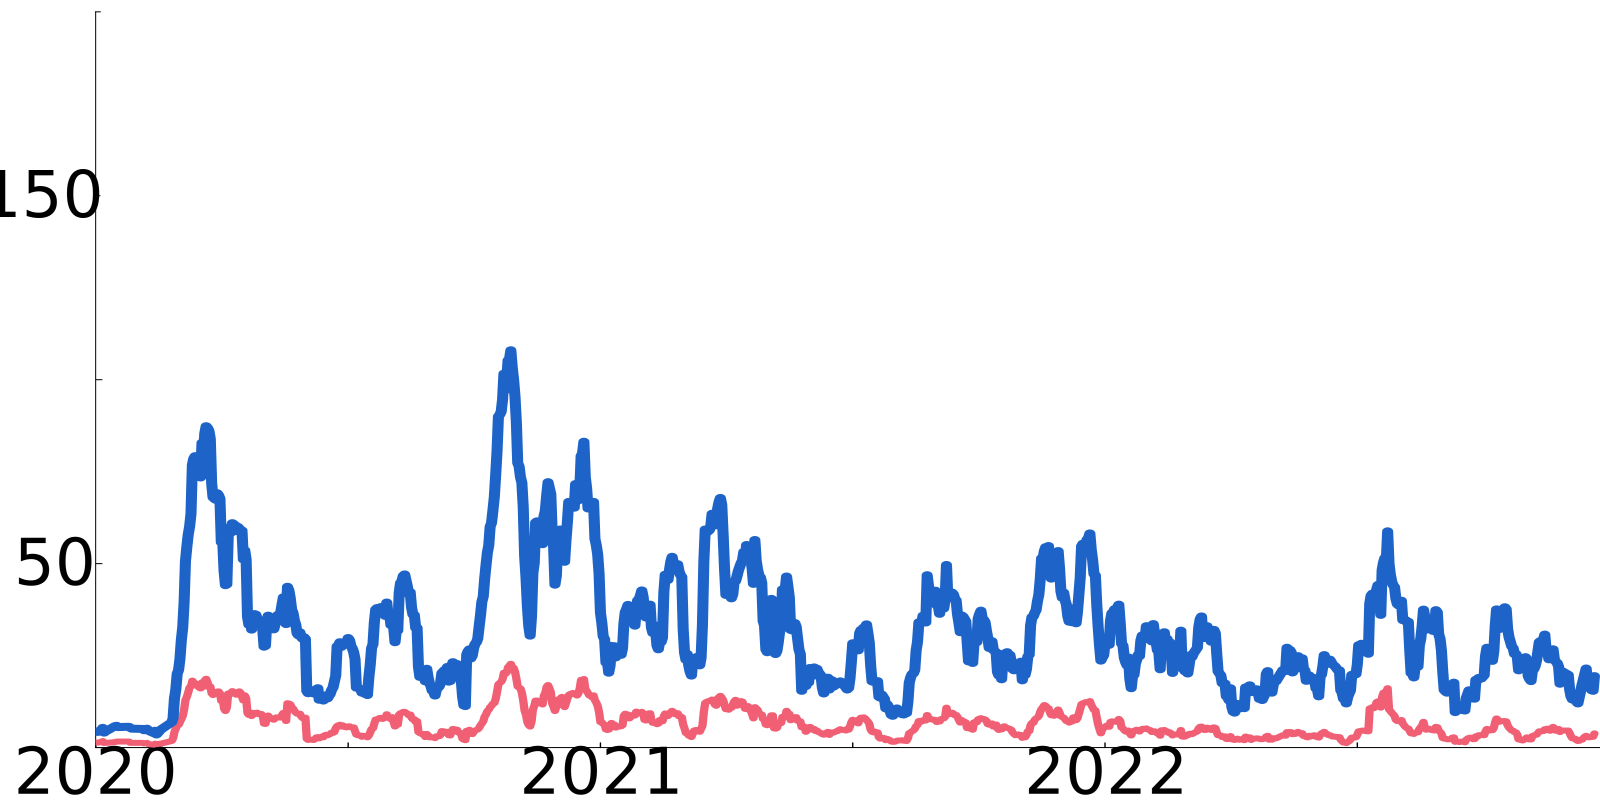
\includegraphics[width=.8\textwidth]{figures/reddit/lockdown}}
			\only<2>{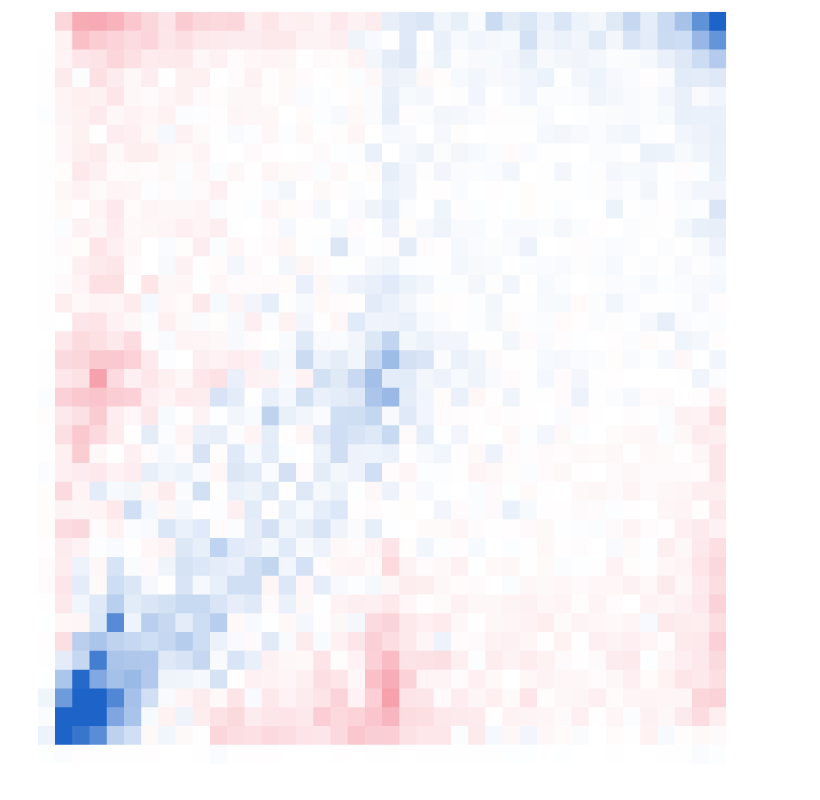
\includegraphics[width=.6\textwidth]{figures/reddit/sentiment}}
			\only<3>{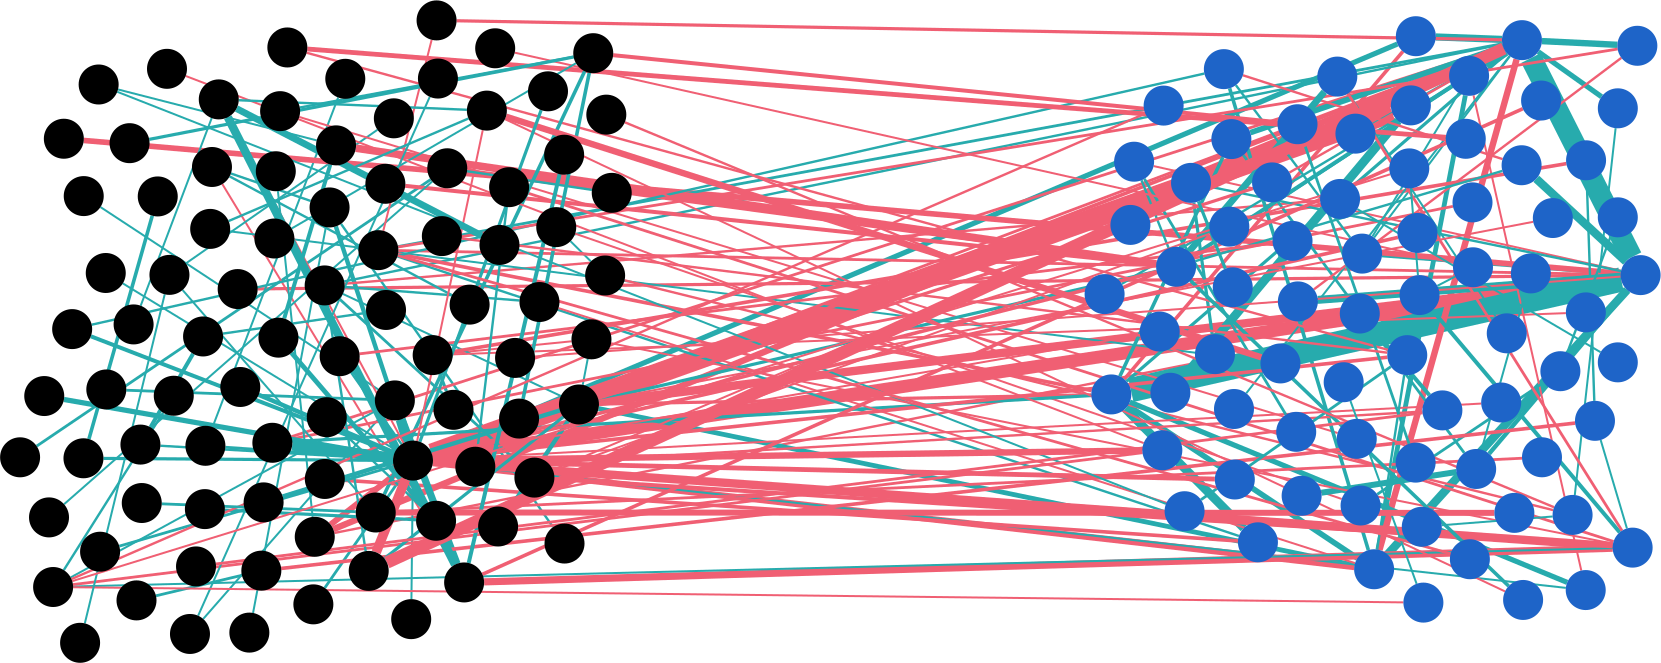
\includegraphics[width=.8\textwidth]{figures/reddit/network}}
		\end{column}
	\end{columns}
\end{frame}

\begin{frame}{The Dataset}
	\twocolumns{%
		\begin{itemize}
			\item r/Belgium community
			\item 01/2020 - 07/2022
			\item COVID topics by keyword selection and pretrained BERT model
			\begin{itemize}
				\item Lockdown
				\item Mask
				\item Vaccination
			\end{itemize}
			\item Sentiment by pretrained BERT model
		\end{itemize}
	}{%
		\centering
		\scalebox{0.75}{
			\begin{tabular}{rccc}	\hline
															& \tabhead{Users} & \tabhead{Comments} & \tabhead{Submissions} \\\hline
				\textbf{Total}        & 28559 & 645280   & 10362 \\
				Lockdowns     & 9987  & 94494    & 1009 \\
				Masks         & 6824  & 48500    & 437 \\
				Vaccination   & 5552  & 41700    & 590 \\
			\end{tabular}
		}
	}
\end{frame}


% \begin{frame}
% 	\vspace{10pt}
% 	\only<1>{\begin{tikzpicture}
% 	  \focusedlockdown
% 	  \unfocusedmask
% 	  \unfocusedvaccin
% 	\end{tikzpicture}}
% 	\only<2>{\begin{tikzpicture}
% 	  \unfocusedlockdown
% 	  \focusedmask
% 	  \unfocusedvaccin
% 	\end{tikzpicture}}
% 	\only<3->{\begin{tikzpicture}
% 	  \unfocusedlockdown
% 	  \unfocusedmask
% 	  \focusedvaccin
% 	\end{tikzpicture}}
% 	\only<4>{
% 		\vspace{-240pt}
% 		\begin{center}
% 			\begin{tikzpicture}
% 				\node[] {%
% 					\includegraphics[width=.8\textwidth]{figures/pics/vaccine}
% 				};
% 			\end{tikzpicture}
% 		\end{center}
% 	}
% 	\focusedlockdown
% 	\focusedmask
% 	\focusedvaccin
% \end{frame}

\begin{frame}{Topic contagion}
	\twocolumns[.5]{%
		\begin{itemize}
			\item Can participating in a discussion \alert{cause} a user to initiate one?
			\item Post is \alert{initiating} if no ancestor shares the same topic
			\item Else, participating
		\end{itemize}
	}{%
		\begin{tikzpicture}
			\contagionexample
		\end{tikzpicture}
	}
\end{frame}

\begin{frame}{No evidence of topic contagion}
	\twocolumns[.5]{%
		\begin{tikzpicture}
			\activitycdf[ecdfylabels]{lockdown}{\addactivitylegend}
		\end{tikzpicture}
		\begin{itemize}
			\item Lockdowns
		\end{itemize}
	}{%
		\begin{tikzpicture}
			\activitycdf[]{vaccin}{}
		\end{tikzpicture}
		\begin{itemize}
			\item Vaccination
		\end{itemize}
	}
	\begin{itemize}
		\item \alert{Observed $\rho(i)$ lies above null} at small $i$: initiations occur \emph{earlier} than expected
		\item Participating does not lead to initiating
	\end{itemize}
\end{frame}

\begin{frame}{Sentiment interactions: vaccination}
  \twocolumns{%
    \begin{tikzpicture}
      \sentheatmap{vaccin}
    \end{tikzpicture}
		\begin{itemize}
			\item \alert<1>{Homophily!}
			\item Replies have similar levels as parent
		\end{itemize}
  }{%
    \begin{tikzpicture}
      \only<2-3>{\vertextree}
      \only<2>{\structurededges}
      \only<3>{\randomedges}
      \only<4>{\diffheatmap{vaccin}}
    \end{tikzpicture}
		\begin{itemize}
			\item<2-> Expected if everyone is negative
			\item<3-> Compare to random realisation
			\item<4-> \alert{Homophily confirmed}
		\end{itemize}
  }
\end{frame}

\begin{frame}{SIEBC Model}
	\twocolumns[.3]{%
		\begin{itemize}
			\item \textbf{S}mooth
			\item \textbf{I}nternal-\textbf{E}xpressed
			\item \textbf{B}ounded \textbf{C}onfidence
		\end{itemize}
	}{%
		\begin{align*}
			e_i[t] & \sim B_{{\only<2>{\color{color1}}\alpha_{e,i}}, \epsilon_i}(u_i[t-1], {\only<1>{\color{color1}} e_j[t]})\\
			u_i[t] & \sim {\only<1>{\color{color2}}\bigotimes_{e_{k}\in I_i[t-1]}} B_{{\only<2>{\color{color2}}\alpha_{u,i}}, \epsilon_i}(u_i[t-1], {\only<1>{\color{color2}} e_{k}})
		\end{align*}
	}
	\vspace{24pt}
	\newcommand{\annotationsize}{\small}
\begin{tikzpicture}
  %% DIAGRAM

  \begin{scope}[shift={(0pt,0)}]
    % Subfigure
    % Nodes
    \node at (0,0) (U) {\( u_i[t] \)};
    \node at (3.4,0) (Ut) {\( u_i[t+1] \)};
    \node at (0, 2.4) (E) {\( e_i[t] \)};
    \node at (-2, 1.2) (P) {\only<1>{\color{color1}}\( e_j[t] \)};
    \node at (1.8, 1.2) (R1) {\only<1>{\color{color2}}\( e_{1} \)};
    \node at (3, 1.2) (RK) {\only<1>{\color{color2}}\( e_{k} \)};

    % Edges
    \only<1>{\draw[->] (U) -- (E);}
    \only<2>{\draw[->, color1, line width=1.2pt] (U) -- (E);}
    \only<1>{\draw[->] (P) -- (E);}
    \only<2>{\draw[->, color1, line width=1.2pt] (P) -- (E);}
    \draw[->] (P) -- (U);
    \draw[->] (E) -- (R1);
    \draw[->] (E) -- (RK);
    \only<1>{\draw[->] (R1) -- (Ut);}
    \only<2>{\draw[->, color2, line width=1.2pt] (R1) -- (Ut);}
    \only<1>{\draw[->] (RK) -- (Ut)};
    \only<2>{\draw[->, color2, line width=1.2pt] (RK) -- (Ut);}
    \only<1>{\draw[->] (U) -- (Ut);}
    \only<2>{\draw[->, color2, line width=1.2pt] (U) -- (Ut);}

    % Annotations
    \node at (0, -.4) {\annotationsize Internal};
    \node at (0, 2.8) {\annotationsize Expressed};
    %\node at (-1.9, 2.2) {\annotationsize Focal user};

    \node at (2.4, 1.2) {\only<1>{\color{color2}}\( \cdots \)};
    \node[align=center] at (3, 2.2) {\annotationsize \only<1>{\color{color2}} Replied sentiments \\ \only<1>{\color{color2}} \( I_i[t, t+1] \)};
    \node[align=center] at (-2, 2.05) {\annotationsize \only<1>{\color{color1}} Parent \\ \only<1>{\color{color1}}sentiment};
    \node[align=center] at (-0.85, 1.6) {\annotationsize \( \only<2>{\color{color1}} \alpha_{e,i} \) };
    \node[align=center] at (2.85, 0.72) {\annotationsize \( \only<2>{\color{color2}} \alpha_{u,i} \)};
  \end{scope}
  %% Reddit thread
  \only<1>{\node at (13.5,1.5) {%
    \begin{minipage}[t]{\textwidth}
      \dirtree{%
        .1 \color{color1} Parent expression.
          .2 Focal expression.
            .3 \color{color2} Reply expression.
            .3 \color{color2} Reply expression.
              .4 \color{color2bw} Irrelevant expression.
      }
    \end{minipage}
  };}
  %% 1D KERNEL
  \only<2->{\begin{axis}[
    xshift=205pt,
    yshift=0pt,
    width=.333\textwidth,
    height=.3\textwidth,
    axis lines*=left,
    %
    xmin=-1,
    xmax=1,
    xlabel=\( s_2 - s_1 \),
    xtick={-1, -0.33, 0, 0.33, 1},
    xticklabels={-1, -\( \epsilon \), 0, \( \epsilon \), 1},
    %
    ymin=-.4,
    ymax=.4,
    ylabel=\( B_{\alpha, \epsilon} \),
    ylabel style={%
      at={(axis description cs:-0.05,1.15)},
      anchor=north,
      rotate=-90,
    },
    ytick={-0.3, 0, 0.3},
    yticklabels={\( s_1 -\alpha\cdot\epsilon \), \( s_1 \), \( s_1 + \alpha\cdot\epsilon \)},
    %
  ]
    \addplot[
      mark=none,
      line width=2pt,
      color=color2,
    ]
    table[x=x, y=y2, col sep=comma]{figures/siebc/kernel1d.csv};

    \addplot[
      mark=none,
      line width=2pt,
      color=color1,
    ]
    table[x=x, y=y1, col sep=comma]{figures/siebc/kernel1d.csv};
  \end{axis}}
\end{tikzpicture}
\end{frame}

\newcommand{\topiccol}[2]{%
	\begin{column}{.33\textwidth}
		\begin{tikzpicture}
			#1
		\end{tikzpicture}
		\begin{itemize}
			\item #2
		\end{itemize}
	\end{column}
}

\begin{frame}{Reconstruction of sentiment distributions}
	\begin{columns}
		\topiccol{\modelsentiment{lockdown}{}}{Lockdowns}
		\topiccol{\modelsentiment{mask}{}}{Masks}
		\topiccol{\modelsentiment{vaccin}{\addmodellegend}}{Vaccination}
	\end{columns}
	\begin{itemize}
		\item Okay attempt at predicting difficult distributions
		\item Homophily present in predicted sentiments as well
	\end{itemize}
\end{frame}

\begin{frame}{Expressed sentiment update is strongest}
	\begin{columns}
		\topiccol{\modelalphas[]{lockdown}{0.41037}{0.88267}{}}{Lockdowns}
		\topiccol{\modelalphas[]{mask}{0.41230}{0.66326}{}}{Masks}
		\topiccol{\modelalphas[]{vaccin}{0.41677}{0.51952}{\alphaslegend}}{Vaccination}
	\end{columns}
	\begin{itemize}
		\item Expressed sentiment might diverge from actual sentiment
	\end{itemize}
\end{frame}

\begin{frame}{Strengths of SIEBC}
	\begin{itemize}
		\item Bounded confidence kernel is required to explain homophily (cfr. \( L_\alpha \) )
		\item Hidden state can deal with nois (cfr. $\bar{e}$)
	\end{itemize}
	\centering
	\vfill
	\begin{tabular}{lccccccccc}\hline
		& \multicolumn{2}{c}{\emph{Lockdowns}} & \multicolumn{2}{c}{\emph{Masks}} & \multicolumn{2}{c}{\emph{Vaccination}} \\
		\textbf{Model} & \( KS \) & \( \Delta h \) & \( KS \) & \( \Delta h \) & \( KS \) & \( \Delta h \) \\ \hline
		\( L_\alpha \) & 0.044 & -0.097 \( \pm 0.009 \) & 0.048 & -0.131 \( \pm 0.017 \) & 0.068 & -0.103 \( \pm 0.018 \) \\
		\( \bar{e} \) & 0.049 & -0.070 \( \pm 0.023 \) & 0.052 & -0.075 \( \pm 0.033 \) & 0.076 & -0.056 \( \pm 0.047 \) \\
		SIEBC  & \textbf{0.043} & \textbf{-0.027} \( \pm 0.013 \) & \textbf{0.043} & \textbf{-0.067} \( \pm 0.020 \) & \textbf{0.055} & \textbf{-0.033} \( \pm 0.021 \) \\\hline
	\end{tabular}
	\vfill
\end{frame}

\begin{frame}{Conclusions}
	\twocolumns{%
		\only<1->{\begin{itemize}
			\item Simple model explains complex data
			\item Sentiment is not a very meaningful signal
			\item Reddit is not a representative sample
		\end{itemize}}
	}{%
		\only<2>{\begin{itemize}
			\item Topics discussed depends on external factors
			\item BC model can explain homphily
			\item (Subtle) differences exist between topics
		\end{itemize}}
	}
\end{frame}

\end{document}
